\documentclass[11pt]{amsbook}

\usepackage{../HBSuerDemir}	% ------------------------

\begin{document}

% ++++++++++++++++++++++++++++++++++++++
\hPage{b1p2/482}
% ++++++++++++++++++++++++++++++++++++++

\subsection{Volume of a Solid of Revolution}:
\label{subsec:VolumeofaSolidofRevolution}
\\
A \hDefined{solid of revolution} is the solid generated by revolving a plane region about a (straight) line. This line is called the symmetry axis of the solid. The boundary of a surface of revolution is certainly a surface of revolution.
\\
Consider first a region under the curve of a continuous positive function \(y=f(x)\) bounded by the lines \(x=a, x=b.\)
\\
When this region is revolved about the x-axis (or the y-axis), it generates a solid of revolution whose volume is denoted by \(V_{ox}\) (or \(V_{oy}\)).
\begin{figure}[htb]
	\centering
    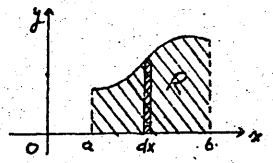
\includegraphics[width=.4\textwidth]{images/b1p2-482-fig01}
\end{figure}
\\
For this region, for convenience \(V_{ox}\) will be evaluated by what we call \hDefined{disc method}, while \(V_{oy}\) by \hDefined{shell method} as explained below.
\\
Consider an element of area as a vertical strip in the region R. When R is rotated about x-axis (y-axis) the strip generates an element of volume in the form of a \hDefined{disc} (a \hDefined{shell})
\begin{figure}[htb]
	\begin{minipage}{0.45\textwidth}
		\centering
    	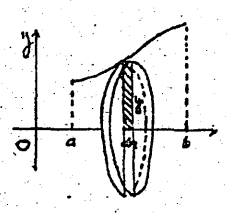
\includegraphics[width=\textwidth]{images/b1p2-482-fig02}
		\caption{Disc of radius y and thickness dx}
	\end{minipage}
	\begin{minipage}{0.45\textwidth}
		\centering
    	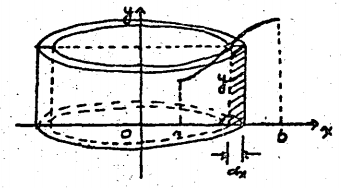
\includegraphics[width=\textwidth]{images/b1p2-482-fig03}
		\caption{Shell of inner radius x, thickness dx and height y.}
	\end{minipage}
\end{figure}

% =======================================================
\end{document}  

%==== templates ====

%==== environments ====

%\begin{figure}[htb]
%	\centering
%	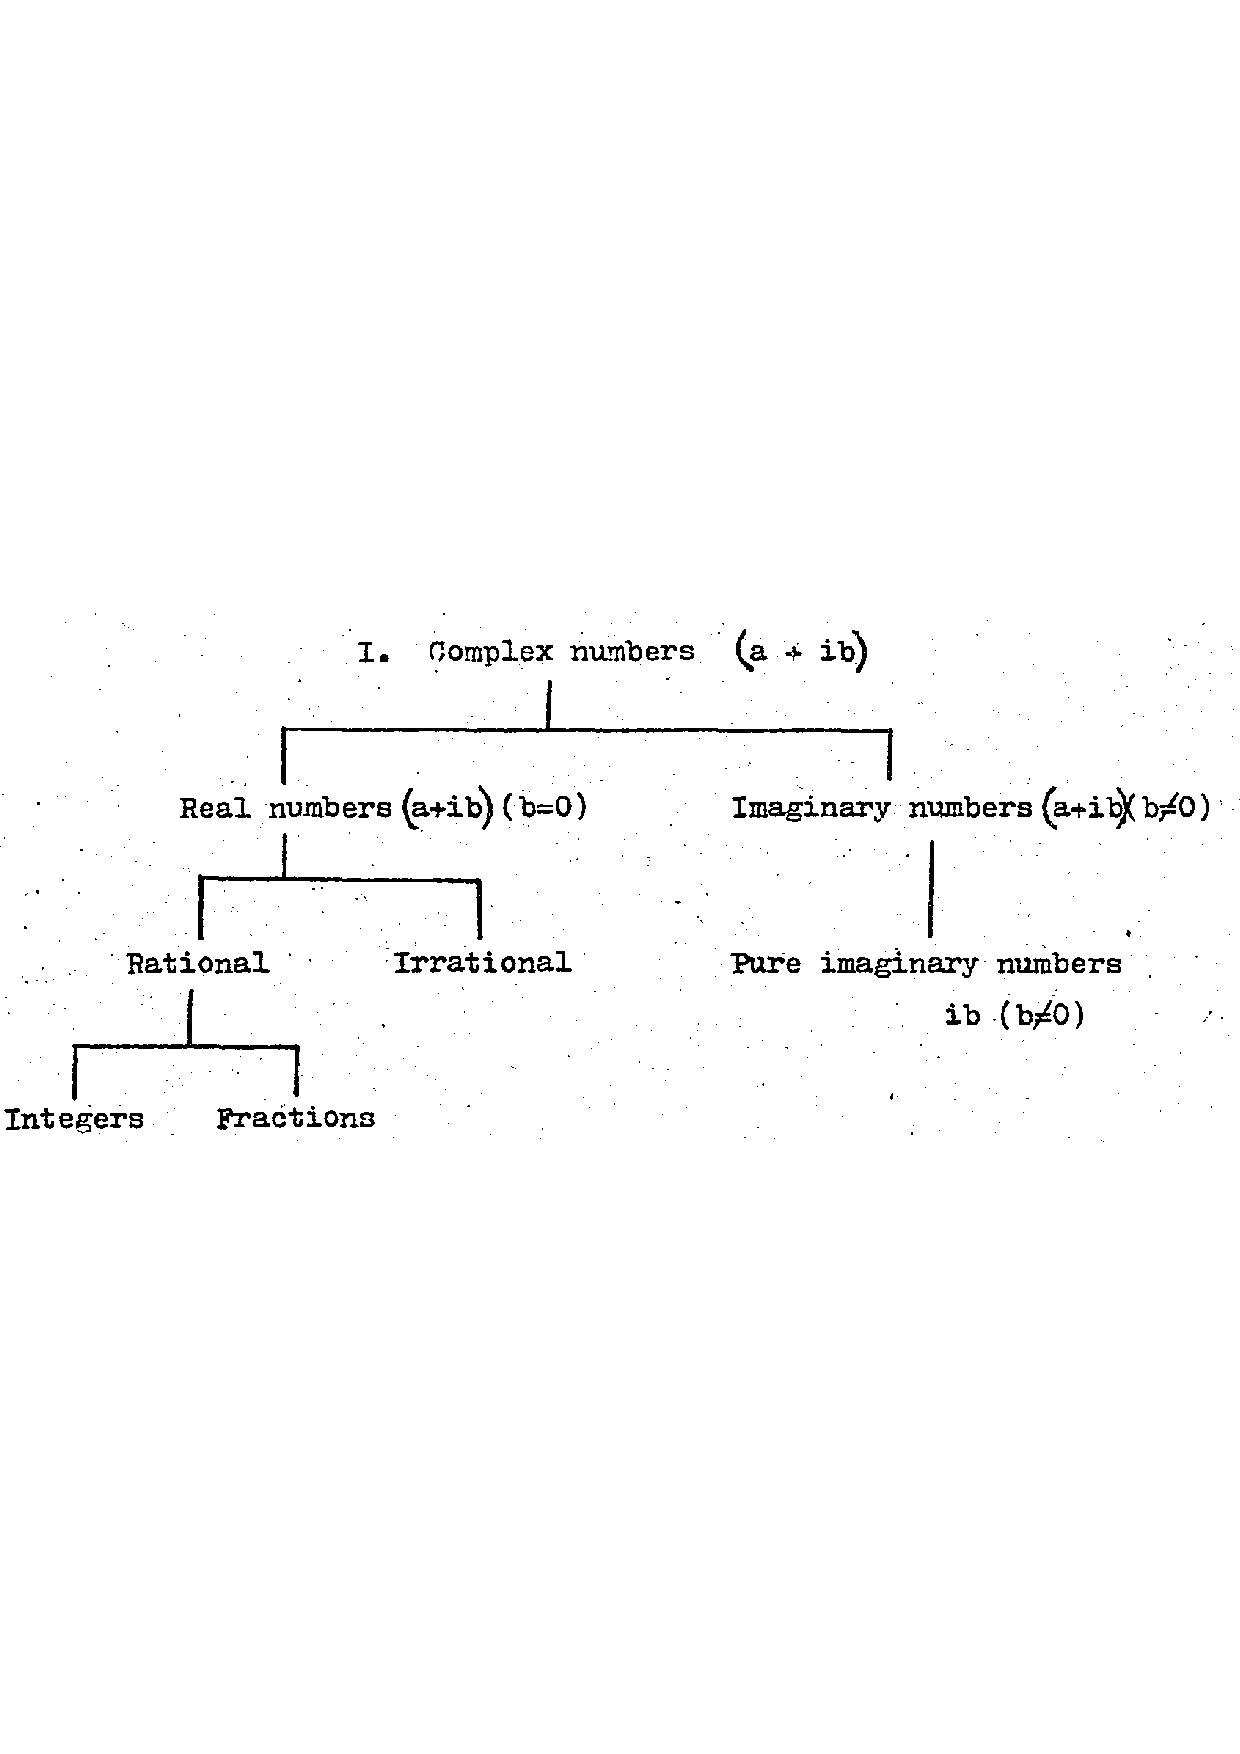
\includegraphics[width=0.9\textwidth]{images/SD-1-1p15A}
%	\caption{Classification of complex numbers}
%	\label{fig:classificationOfComplexNumbersA}
%\end{figure}

%\begin{center}
%\begin{tabular}{cc}
%\end{tabular}
%\end{center}

%\begin{exmp}
%\begin{hSolution}
%\end{hSolution}
%\end{exmp}

%\begin{hEnumerateAlpha}
%\end{hEnumerateAlpha}

%\begin{hEnumerateRoman}
%\end{hEnumerateRoman}

%$
%\begin{bmatrix}
%\end{bmatrix}
%$

%\frac{aaaa}{bbb}
%\frac{a_{n}}{b_{n}}
%\left( aaaa \right)
%\Longrightarrow

%\begin{multicols}{2}
%	bb
%\columnbreak
%	aa
%\end{multicols}
